\documentclass[11pt,a4paper]{article}

\usepackage[utf8]{inputenc}
\usepackage[T1]{fontenc}
\usepackage{lmodern}
\usepackage[margin=1.9cm,headheight=14pt,headsep=7mm,footskip=10mm]{geometry}
\usepackage{graphicx}
\usepackage{booktabs}
\usepackage{array}
\usepackage{tabularx}
\usepackage{longtable}
\usepackage{enumitem}
\usepackage{titlesec}
\usepackage{fancyhdr}
\usepackage{caption}
\usepackage{amsmath}
\usepackage{amssymb}
\usepackage{tikz}
\usepackage{xcolor}
\usepackage{microtype}
\usepackage[hidelinks]{hyperref}
\usetikzlibrary{arrows.meta,positioning,shapes.geometric}

\definecolor{brand}{RGB}{0,77,68}
\definecolor{accent}{RGB}{44,145,112}
\definecolor{muted}{RGB}{93,103,112}
\definecolor{panel}{RGB}{239,246,243}
\definecolor{gridline}{RGB}{210,220,217}

\hypersetup{
  pdftitle={Intelligent Multi-Agent Urban Traffic Management},
  pdfauthor={Esprit 5DS8 Project Team},
  pdfsubject={Advanced Data Science Project - Technical Report}
}

\titleformat{\section}{\Large\bfseries\color{brand}}{\thesection.}{0.55em}{}
\titleformat{\subsection}{\large\bfseries\color{brand}}{\thesubsection}{0.55em}{}
\titleformat{\subsubsection}{\normalsize\bfseries}{\thesubsubsection}{0.55em}{}
\titlespacing*{\section}{0pt}{13pt}{6pt}
\titlespacing*{\subsection}{0pt}{9pt}{4pt}
\titlespacing*{\subsubsection}{0pt}{7pt}{3pt}
\setlist[itemize]{leftmargin=1.35em,topsep=3pt,itemsep=2pt,parsep=1pt}
\setlist[enumerate]{leftmargin=1.6em,topsep=3pt,itemsep=2pt,parsep=1pt}
\setlength{\parindent}{1.1em}
\setlength{\parskip}{2pt}
\setlength{\emergencystretch}{2em}
\captionsetup{font=small,labelfont=bf,skip=4pt}
\renewcommand{\arraystretch}{1.12}

\pagestyle{fancy}
\fancyhf{}
\renewcommand{\headrulewidth}{0.35pt}
\fancyhead[L]{\footnotesize SUMO Traffic-Control Project}
\fancyhead[R]{\footnotesize Esprit 5DS8}
\fancyfoot[C]{\footnotesize\thepage}

\tikzset{
  arch/.style={
    draw=brand,rounded corners=2pt,fill=panel,align=center,
    text width=27mm,minimum height=16mm,inner sep=3.5pt,font=\small
  },
  archwide/.style={arch,text width=29mm},
  archtopdata/.style={arch,fill=white,draw=muted,text width=27mm},
  archdata/.style={arch,fill=white,draw=muted,text width=36mm},
  archagent/.style={arch,fill=accent!12},
  archarrow/.style={-{Latex[length=2.5mm]},line width=0.8pt,draw=brand}
}

\begin{document}

\begin{titlepage}
\thispagestyle{empty}
\centering
\vspace*{1.35cm}
{\large\color{brand}\textbf{ESPRIT SCHOOL OF ENGINEERING}}\\[3pt]
{\normalsize Advanced Data Science Project | 5DS8}\\[1.1cm]
\rule{\textwidth}{1.1pt}\\[9mm]
{\Huge\bfseries\color{brand} Intelligent Multi-Agent\\[3pt] Urban Traffic Management}\\[7mm]
{\Large Technical Report}\\[3mm]
{\large SUMO simulation, traffic-signal control, and reproducible baseline evaluation}\\[9mm]
\rule{\textwidth}{0.55pt}\\[11mm]

\begin{tabular}{>{\bfseries}rl}
Project name: & SUMO Traffic-Control Research and Dashboard \\
Course: & Advanced Data Science Project \\
Supervisor: & Islem Maiti \\
Team: & Hazem Mrad, Bilel Brini, Lina Haddad,\\
      & Amen Allah Ben Aissa, Rami Ben Slimen \\
Study network: & Generated San Francisco Mission 2$\times$2 grid \\
Evidence in this report: & 30 exploratory SUMO episodes; 3 classical controllers \\
\end{tabular}

\vfill
\begin{minipage}{0.88\textwidth}
\small
\textbf{Scope note.} This report distinguishes the project's implemented MARL framework
from the specific measured experiment reported here. The quantitative comparison is a
short-horizon study of fixed-time, actuated, and Max-Pressure controllers. It does not
evaluate a learned PPO policy and is not evidence of real-world traffic improvement.
\end{minipage}
\vspace{12mm}
\end{titlepage}

\pagenumbering{roman}
\section*{Abstract}
\addcontentsline{toc}{section}{Abstract}
Urban signal control is a multi-objective problem: reducing delay and queues must be
balanced against throughput, emissions, pedestrian service, and emergency response.
This project builds an end-to-end research and demonstration system around Eclipse SUMO.
Its Python domain contains a PettingZoo parallel multi-agent environment, classical
controllers, a parameter-shared PPO training path, a rule-based safety shield, metric
collection, and a FastAPI service connected to a Vite operations dashboard.

To provide auditable quantitative evidence, we ran a paired exploratory comparison of
three non-learned controllers on a generated four-intersection grid: Webster fixed-time
(\texttt{ft}), gap-actuated (\texttt{act}), and Max-Pressure (\texttt{mp}). The experiment
crossed two event settings (normal and emergency), one medium-demand level, and five
shared random seeds, for 30 episodes. Each quick-mode episode used a 300-second warm-up,
a 600-second measured interval, and a 300-second cooldown. In both event settings, the
actuated controller had the lowest mean waiting time (6.69 s normal; 6.72 s emergency),
while Max-Pressure had the lowest CO$_2$ intensity (211.73 and 215.82 g/km) and marginally
higher throughput. The results are descriptive pilot evidence only: one small network,
one demand level, five seeds, and no significance testing.

\noindent\textbf{Keywords:} SUMO, intelligent transportation, traffic signals, MARL, PPO,
Max-Pressure, reproducible evaluation, urban mobility.

\section*{Executive Summary}
\addcontentsline{toc}{section}{Executive Summary}
\begin{itemize}
  \item \textbf{Problem:} fixed plans cannot respond to changing queues and event-driven
  demand, while unconstrained adaptive control can create unsafe or unfair signal timing.
  \item \textbf{Approach:} model one agent per signalised junction; share observations and
  optional neighbour information; place a deterministic timing shield between proposed
  and executed phases; evaluate controllers in SUMO.
  \item \textbf{Pilot result:} actuated control reduced mean waiting relative to
  Max-Pressure by about 24\% in this quick-mode sample, with a small CO$_2$-intensity
  trade-off. Max-Pressure retained slightly higher throughput. Fixed-time performed
  worst on mean delay in these runs.
  \item \textbf{Evidence boundary:} these are classical-controller results, not a learned
  policy comparison. Results are not statistically significant claims or field estimates.
  \item \textbf{Readiness:} the backend, UI, experiment configuration, run-level CSV,
  aggregate table, manifest, and test/build evidence are available in the repository.
\end{itemize}

\newpage
\tableofcontents
\newpage
\pagenumbering{arabic}

\section{General Context}
Road traffic at signalised intersections is a dynamic system. Vehicles arrive in
bursts, queues spill back, turning flows compete for green time, and unusual events
such as emergency vehicles or pedestrian demand change what an appropriate signal plan
should do. Decisions at adjacent intersections are coupled: releasing traffic from one
junction changes the arrival pattern at the next. A single fixed signal plan is
therefore an imperfect response to all operating conditions.

Microscopic traffic simulation provides a controlled environment for studying this
problem. Eclipse SUMO [1] represents individual vehicles, road lanes, traffic lights, trips,
and emissions. It makes it possible to vary traffic demand and random seeds while
observing the consequences of candidate controllers. It does not, by itself, establish
that a controller will work in a real city: conclusions remain conditional on the
network, demand model, vehicle behaviour, and simulated operating horizon.

The project combines a research pipeline with an operator-facing dashboard for SUMO.
The research layer owns the environment, policies, experiment configuration, and
metrics. The dashboard presents a live simulation and results-oriented views; it is
not a source of independent traffic measurements. This separation is important for
reproducibility: the reported metrics are generated by the SUMO evaluation pipeline,
not inferred from a screenshot or from an external live traffic feed.

\subsection{Project vision}
The motivating question is: \emph{How can data and intelligent agents make urban
traffic management more efficient, adaptive, and sustainable without compromising
operational constraints?} The intended long-term application supports traffic
operators with interpretable monitoring and decision support. The present prototype
is a simulation research system, not an autonomous city deployment.

\section{Problem Statement and Scope}
\subsection{Problem statement}
Given a network of signalised intersections and time-varying demand, select signal
phases so that traffic moves efficiently while critical movements are not starved and
pedestrians and emergency vehicles remain represented in the control objective. The
controller receives simulated observations at discrete decision times and proposes a
green phase for each junction. The simulator then advances the network and records
system-level outcomes.

The central methodological challenge is not simply to minimise average waiting. An
optimisation that improves mean delay could still worsen the upper tail, emissions,
throughput, or priority for vulnerable road users. A sound comparison must therefore
state its operating conditions, use consistent seeds across controllers, measure
multiple outcomes, and discuss trade-offs rather than naming a universal winner.

\subsection{Research question and pilot scope}
The quantitative question addressed here is intentionally narrow:
\begin{quote}
\textbf{RQ1.} On the generated \texttt{grid2x2} network at medium demand, how do
fixed-time, actuated, and Max-Pressure controllers compare on delay, throughput,
queueing, and simulated CO$_2$ intensity under normal and emergency event settings?
\end{quote}

This pilot does \emph{not} answer whether PPO or another MARL algorithm outperforms
classical control, whether the result generalises to Monaco or Tunis, or whether the
system improves real-world safety. The repository includes larger networks and a
generalist PPO recipe, but a sufficiently controlled learned-policy comparison is
outside the measured scope of the 30 episodes reported in this document.

\section{Proposed Solution and Ideation Objectives}
\subsection{Proposed solution}
The proposed system uses SUMO as the controlled experimental environment and
\texttt{CoTrafficEnv} as the common interface for controllers. In the MARL path, each
signalised intersection is an agent. The agents act in parallel and share a policy
architecture; configured observation blocks provide local traffic state and, for
cooperative variants, neighbouring or special-user information. Every learned or
pressure-based action passes through a rule-based safety shield before it is executed.
Classical signal plans use the same simulation and metric pipeline, creating a common
basis for later comparisons.

The operator-facing SUMO dashboard complements the research path. The FastAPI
backend exposes policy, simulation, and result endpoints. The Vite frontend displays a
map context, key counters, trend plots, event information, and live-run status. The
interface supports a demonstration workflow; numerical claims in this report are taken
from saved experiment artifacts instead.

\subsection{Business objectives (BO)}
The business objectives are project goals for a future traffic-operations use case, not
measured outcomes from a deployed traffic agency.
\begin{enumerate}
  \item \textbf{BO1 - Reduce avoidable delay:} improve how green time responds to
  observed demand, using mean and tail delay as complementary measures.
  \item \textbf{BO2 - Preserve network service:} avoid trading local gains for reduced
  completed trips or lower corridor throughput.
  \item \textbf{BO3 - Support priority and access:} represent emergency vehicles,
  pedestrians, and buses in the observations, rule overlays, and/or objective.
  \item \textbf{BO4 - Make operations inspectable:} present run status, controller,
  traffic counters, events, and experiment results in a single control-room interface.
  \item \textbf{BO5 - Enable reproducible improvement:} keep networks, scenarios,
  recipes, seeds, and timing parameters in versioned configuration files.
\end{enumerate}

\subsection{Data science objectives (DSO)}
\begin{enumerate}
  \item \textbf{DSO1 - Build a repeatable simulator dataset:} generate episodes from
  explicit network, demand, event, and seed configurations.
  \item \textbf{DSO2 - Define a multi-agent control formulation:} map junction state to
  discrete phase actions and compute configurable, normalised reward components.
  \item \textbf{DSO3 - Compare against credible baselines:} establish fixed-time,
  actuated, and Max-Pressure reference behaviour before claiming a learned-policy gain.
  \item \textbf{DSO4 - Measure trade-offs:} report delay, tail delay, queue, throughput,
  emissions intensity, and completion/safety indicators together.
  \item \textbf{DSO5 - Preserve evidence provenance:} save each episode's metrics,
  aggregate results, experiment settings, software versions, and validation status.
\end{enumerate}

\begin{longtable}{>{\bfseries\raggedright\arraybackslash}p{1.8cm}
                  >{\raggedright\arraybackslash}p{4.7cm}
                  >{\raggedright\arraybackslash}p{9.2cm}}
\caption{Relationship between all project objectives, indicators, and the pilot evidence.}
\label{tab:objective-evidence}\\
\toprule
\textbf{Objective} & \textbf{Intended indicator} & \textbf{Evidence and scope in this report} \\
\midrule
\endfirsthead
\multicolumn{3}{l}{\small\itshape Table~\ref{tab:objective-evidence} continued}\\
\toprule
\textbf{Objective} & \textbf{Intended indicator} & \textbf{Evidence and scope in this report} \\
\midrule
\endhead
\midrule
\multicolumn{3}{r}{\small\itshape Continued on next page}\\
\endfoot
\bottomrule
\endlastfoot
BO1 & Reduce avoidable delay: mean and tail waiting time &
Mean and 95th-percentile waiting are reported for all three classical controllers. \\
BO2 & Preserve network service: completed trips and throughput &
Throughput and completed-trip counts are reported. This pilot shows small controller differences only. \\
BO3 & Support emergency and pedestrian access &
An emergency-demand scenario is included. Pedestrian demand is not varied in this pilot; no field-safety claim is made. \\
BO4 & Make operations inspectable for an operator &
The dashboard, map views, metrics panels, and live-run controls are illustrated in Figures~\ref{fig:ui-map}--\ref{fig:provided-dashboard2}. \\
BO5 & Enable repeatable and auditable improvement &
The experiment configuration, five paired seeds, episode CSV, aggregate CSV, and provenance manifest are provided. \\
DSO1 & Build a repeatable simulator dataset &
Thirty SUMO episodes were generated on the same configured network, demand level, and seed matrix. \\
DSO2 & Define and implement a multi-agent control formulation &
The report documents the parallel intersection-agent model, discrete phase action, observations, reward configuration, and safety shield. \\
DSO3 & Compare against credible control baselines &
Fixed-time, actuated, and Max-Pressure controllers are compared. The supplied MP--qlearn figure is separate illustrative evidence and is not included in the measured pilot. \\
DSO4 & Measure operational and environmental trade-offs &
Waiting, travel time, tail waiting, queue, throughput, CO$_2$ intensity, and selected operational counters are reported. \\
DSO5 & Preserve experiment provenance &
Run-level records, aggregate summaries, YAML settings, seeds, software versions, and validation status are retained. \\
\end{longtable}

\section{Methodology at a Glance}
The project workflow is summarised below; detailed technical choices and measured
results are described in Sections~\ref{sec:data}--\ref{sec:results}.
\begin{enumerate}
  \item \textbf{Frame the question:} define a network, demand intensity, event condition,
  controller set, and operational metrics.
  \item \textbf{Prepare the simulation:} construct the network and routes, seed the
  demand generator, and apply the configured episode schedule.
  \item \textbf{Control:} at each decision interval, observe local state, select or
  compute a phase, and pass proposed actions through the safety shield.
  \item \textbf{Measure:} run SUMO, collect per-episode outcomes, and retain run-level
  provenance.
  \item \textbf{Compare and communicate:} pair controller runs by seed, aggregate
  descriptive statistics, expose the reproducibility artifacts, and present the SUMO
  dashboard workflow.
\end{enumerate}

\section{Solution Architecture}
\label{sec:architecture}
The architecture has a single simulation and evaluation domain. The CLI and live API
both call the same environment and controller registry rather than implementing a
second traffic simulator in the UI. Configuration files supply network geometry,
demand, scenario events, timing, and model recipes. The batch evaluation path writes
the authoritative experiment outputs; the live path streams a current session snapshot
to the frontend.

\begin{figure}[htbp]
\centering
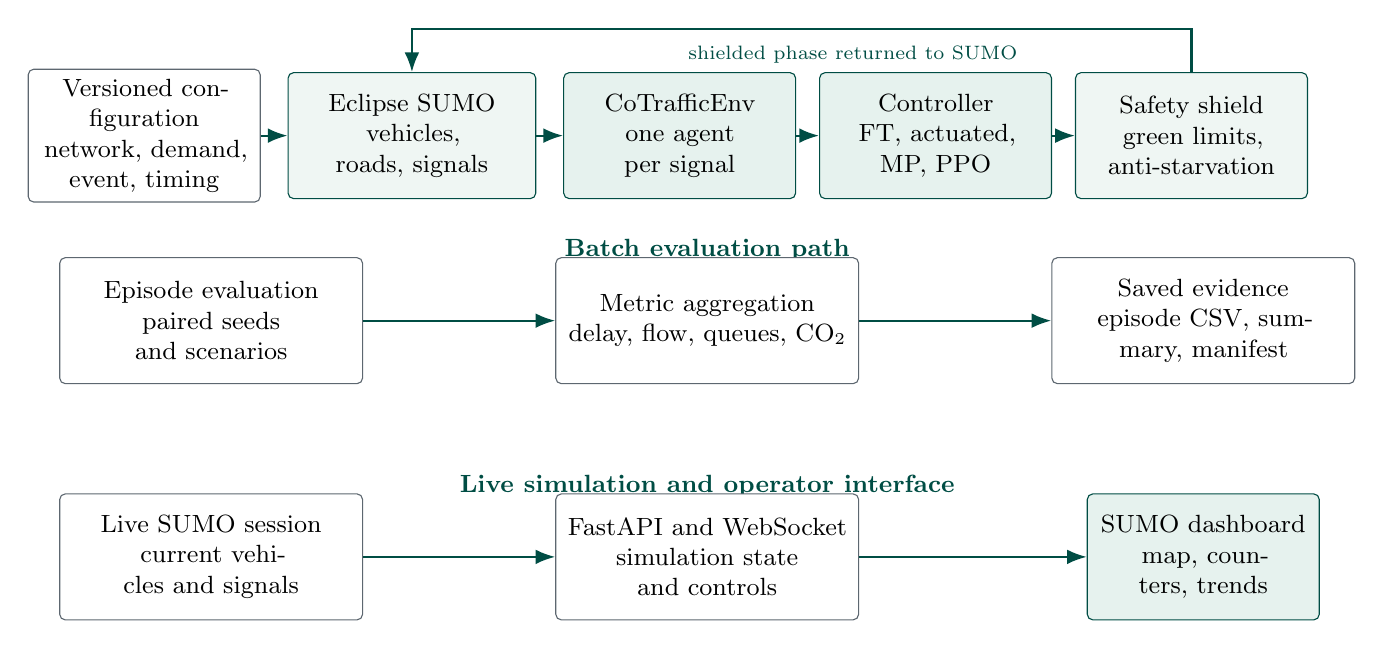
\begin{tikzpicture}[x=1cm,y=1cm]
\node[archtopdata] (cfg) at (1.45,4.2)
  {Versioned configuration\\network, demand, event, timing};
\node[archwide] (sumo) at (4.85,4.2)
  {Eclipse SUMO\\vehicles, roads, signals};
\node[archagent] (env) at (8.25,4.2)
  {CoTrafficEnv\\one agent per signal};
\node[archagent] (policy) at (11.5,4.2)
  {Controller\\FT, actuated, MP, PPO};
\node[arch] (shield) at (14.75,4.2)
  {Safety shield\\green limits, anti-starvation};
\draw[archarrow] (cfg.east) -- (sumo.west);
\draw[archarrow] (sumo.east) -- (env.west);
\draw[archarrow] (env.east) -- (policy.west);
\draw[archarrow] (policy.east) -- (shield.west);
\draw[archarrow] (shield.north) -- ++(0,0.55) -| (sumo.north);
\node[font=\scriptsize,color=brand] at (10.45,5.23) {shielded phase returned to SUMO};

\node[font=\small\bfseries,color=brand] at (8.6,2.75) {Batch evaluation path};
\node[archdata] (evaluate) at (2.3,1.85)
  {Episode evaluation\\paired seeds and scenarios};
\node[archdata] (metrics) at (8.6,1.85)
  {Metric aggregation\\delay, flow, queues, CO$_2$};
\node[archdata] (records) at (14.9,1.85)
  {Saved evidence\\episode CSV, summary, manifest};
\draw[archarrow] (evaluate.east) -- (metrics.west);
\draw[archarrow] (metrics.east) -- (records.west);

\node[font=\small\bfseries,color=brand] at (8.6,-0.25) {Live simulation and operator interface};
\node[archdata] (session) at (2.3,-1.15)
  {Live SUMO session\\current vehicles and signals};
\node[archdata] (api) at (8.6,-1.15)
  {FastAPI and WebSocket\\simulation state and controls};
\node[archagent] (dashboard) at (14.9,-1.15)
  {SUMO dashboard\\map, counters, trends};
\draw[archarrow] (session.east) -- (api.west);
\draw[archarrow] (api.east) -- (dashboard.west);
\end{tikzpicture}
\caption{Research and demonstration architecture. Batch results are the source of the
reported study metrics; the dashboard displays a separate, transient simulation
session. Straight arrows show the sequence within each path. At each decision step,
the shielded phase is applied back to the SUMO signal; the two lower paths are
separate consumers of the shared simulation domain.}
\label{fig:architecture}
\end{figure}

\subsection{Technology stack}
\begin{itemize}
  \item \textbf{Simulation and networks:} Eclipse SUMO 1.27.1, with generated grids and
  configured real-network assets for separate future studies.
  \item \textbf{Environment and policies:} Python, PettingZoo's parallel API,
  Gymnasium-compatible spaces, NumPy, and the \texttt{cotraffic} domain package.
  \item \textbf{Learning path:} Stable-Baselines3 with SuperSuit vectorisation; PPO [4] is
  the configured generalist recipe, and DQN is available as a comparison algorithm.
  \item \textbf{Service and interface:} FastAPI and WebSockets for the live run;
  Vite-based frontend and Mapbox GL for the map presentation.
  \item \textbf{Experiment records:} YAML configuration, CSV episode and aggregate
  tables, JSON manifest, and automated Python/frontend tests.
\end{itemize}

\section{Data and Simulation Environment}
\label{sec:data}
\subsection{Data origin and preparation}
The reported experiment uses \emph{synthetic, simulator-generated data}. SUMO's demand
generator creates trips and routes from the network and demand configuration. The
normal condition contains demand without an added event. The emergency condition
introduces three to five emergency vehicles per seed during the measured hour (with
event times scaled for quick mode). Seeds 0--4 control the random realisations. No
municipal sensor feed, personally identifiable information, or real-world traffic
observation is used in the pilot.

The \texttt{grid2x2} network is a generated toy network for fast debugging and
validation. It has a 2-by-2 arrangement of four signalised intersections, two lanes
per side, 250 m grid links, and pedestrian infrastructure. It is not the Monaco or
Tunis OpenStreetMap network and should not be described as a field deployment. The
dashboard screenshot uses a map backdrop for operator context; the study metrics come
from the generated SUMO network and demand.

\subsection{Episode and decision timing}
The shared protocol advances SUMO in one-second simulation steps. A controller
decision is made every five simulated seconds. Yellow transitions last three seconds;
the default safety limits are a minimum green of ten seconds, a maximum green of
60 seconds, and a 90-second maximum red threshold for anti-starvation.

\begin{table}[htbp]
\centering\small
\caption{Pilot episode design and protocol settings.}
\begin{tabularx}{\textwidth}{>{\bfseries}p{4.0cm}X}
\toprule
Setting & Value \\
\midrule
Network & \texttt{grid2x2}; generated four-intersection network \\
Demand & Medium; same configured intensity for all three controllers \\
Event conditions & Normal and emergency \\
Controller methods & \texttt{ft}, \texttt{act}, \texttt{mp} \\
Seeds & 0, 1, 2, 3, 4; same seed set within each scenario \\
Episodes & $2 \times 3 \times 5 = 30$ total runs \\
Warm-up & 300 s, excluded from measured outcomes \\
Measurement window & 600 s \\
Cooldown & 300 s, to allow trips from the measured window to finish \\
Decision interval & 5 s; SUMO step length 1 s \\
\bottomrule
\end{tabularx}
\end{table}

\subsection{Preparation and measurement}
Each episode is assembled from a network, demand level, event scenario, protocol, and
seed. The evaluation pipeline executes the controller, measures the configured
outcomes, and writes a CSV record. Aggregation groups episodes by network, scenario,
demand, and controller. The results table reports the across-seed sample mean and
sample standard deviation. For the controller comparison, seed-matched differences
are also summarised relative to Max-Pressure.

\begin{itemize}
  \item \textbf{Primary outcome:} mean vehicle waiting time in seconds.
  \item \textbf{Secondary service measures:} mean travel time, 95th-percentile waiting,
  mean queue, completed-vehicle throughput per hour, and vehicles represented.
  \item \textbf{Sustainability measure:} simulator CO$_2$ intensity in grams per
  kilometre. It is an output of the SUMO vehicle/emissions model, not a measured
  roadside emissions reading.
  \item \textbf{Operational checks:} collisions, teleports, unfinished trips, and
  vehicles never inserted.
\end{itemize}

\section{Modeling and Traffic-Control Methods}
\label{sec:modeling}
\subsection{Multi-agent formulation}
The environment exposes one agent per signalised intersection through the PettingZoo
[5] parallel API. At a decision boundary, each agent receives a fixed-size observation and
selects a discrete phase index. The geometry-specific slots are padded so one
parameter-shared policy can be applied across junctions with compatible configured
observation shapes.

The observation builder can include lane queue, density and speed; current-phase state
and phase pressure; upstream-neighbour messages; emergency-vehicle proximity; waiting
pedestrians; bus occupancy; and predicted inflow. These blocks are configurable rather
than all being present in every recipe. The generalist recipe enables neighbour,
emergency, pedestrian, and bus information; it deliberately omits the optional forecast
block unless the forecasting model is prepared.

\subsection{Learning objective and training path}
The generalist recipe uses parameter-shared PPO. PettingZoo agents are adapted to a
Stable-Baselines3 vector environment with SuperSuit; a shared policy is trained from
experience across the intersection slots. Its configured training scenarios include
normal, emergency, pedestrian, bus, and incident conditions, with low, medium, peak,
and rush-profile demand. The recipe targets 500,000 training timesteps and records
checkpoints periodically.

At a high level, the configurable reward starts from a normalised waiting-time,
queue, or pressure term, then may subtract normalised CO$_2$, emergency-vehicle delay,
and pedestrian-wait penalties. The generalist recipe uses person-weighted delay,
CO$_2$ weight 1.0, emergency weight 2.0, pedestrian weight 1.0, and a reward clip of
5.0. These training weights are design settings, not measured outcomes from the pilot
comparison.

The repository README records a generalist PPO training run to approximately 502,000
steps (seed 1) on the 3-by-3 network, while the learned-controller benchmark remains
pending. This project status must not be confused with the results in Section
\ref{sec:results}: the 30 measured episodes in this report evaluate only classical
controllers on \texttt{grid2x2}.

\subsection{Safety shield}
The controller's requested phase is not necessarily the phase executed by the
environment. A deterministic shield first rejects invalid padded actions, enforces
minimum green, serves a movement that has exceeded the configured red-time threshold,
and prevents indefinite extension of a phase beyond maximum green when another phase
has demand. Yellow is handled by the intersection model rather than requested by the
policy. The shield is a safety constraint for the simulated signal sequence; it is not
a certification of road-user safety in a real installation.

\subsection{Classical baselines}
\begin{description}[leftmargin=3.1cm,style=nextline]
  \item[\texttt{ft} - Fixed-time] Webster-based plan [2], tuned to the demand level using
  the configured calibration procedure.
  \item[\texttt{act} - Actuated] SUMO gap-based actuation, ending a green when the
  configured detector gap is exceeded, subject to the configured minimum and maximum
  greens.
  \item[\texttt{mp} - Max-Pressure] based on the pressure-control method [3]; it selects the phase with the largest sum of incoming
  minus outgoing vehicle counts across its green links; ties retain the current phase.
  Its requested decisions pass through the same safety shield.
\end{description}

\section{Experimental Design and Evaluation}
\subsection{Comparison protocol}
The reproducible configuration is \texttt{configs/experiments/technical\_report\_quick.yaml}.
It runs three controllers across two scenarios on one network and medium demand,
using the same five seed values for each controller within a scenario. Pairing helps
control variation due to random demand, but five seeds are too few to support strong
population-level inference. The quick protocol is intentionally shorter than the
project's full evaluation protocol (which uses a longer warm-up, one-hour measured
period, and cooldown).

\subsection{Analysis plan}
Results are presented as means and sample standard deviations across five episodes.
The primary comparison uses the paired seed-wise difference from Max-Pressure:
\[
\Delta_{\mathrm{wait}} =
\mathrm{wait}_{\mathrm{controller}} -
\mathrm{wait}_{\mathrm{MP}}.
\]
A negative value indicates lower measured waiting than Max-Pressure for that paired
sample. The same descriptive comparison is available for other outcomes. No
hypothesis tests, confidence intervals, or multiple-comparison corrections are
reported. The purpose is to show pilot behaviour and expose trade-offs, not to assert
statistical significance.

\subsection{Validity controls}
\begin{itemize}
  \item All methods use the same network, demand, event configuration, and paired seed
  set within each scenario.
  \item The fixed-time baseline is demand-tuned rather than deliberately weak.
  \item The emergency event condition is reported separately from the no-event
  condition.
  \item The source run records, aggregate summary, YAML configuration, software
  versions, and validation notes are retained.
  \item A controller comparison is not conflated with a live dashboard screenshot.
\end{itemize}

\section{Technical Implementation and Integration}
\subsection{Research software}
The core implementation is organised around \texttt{src/cotraffic}. Environment
construction, observations, reward calculations, network topology, controllers,
training, and evaluation live in this package. Configurations are separated into
network, demand, scenario, protocol, experiment, and recipe files. The controller
registry gives each method one stable identifier, which is used by configuration,
evaluation output, and the API.

\subsection{Service and frontend integration}
FastAPI provides the HTTP boundary. Its live-simulation endpoints start, pause, resume,
step, change speed, and stop a simulation session; state can also be streamed over a
WebSocket. Policy endpoints expose the active controller and its availability. The
Vite dashboard consumes this state to display the map context, counters, traffic
trends, event information, and live-run status. Exported experiment data is served
separately from the transient live simulation state.

\begin{figure}[htbp]
\centering
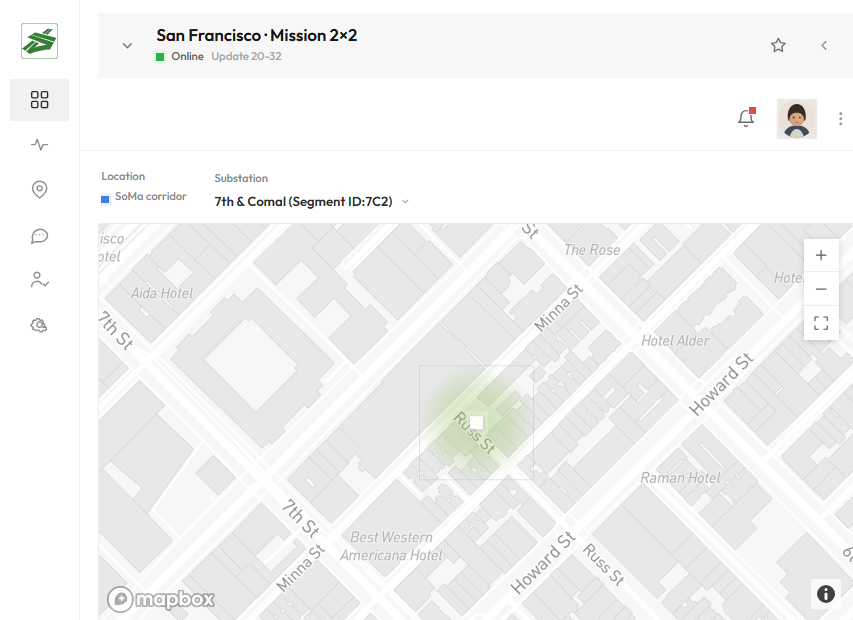
\includegraphics[width=0.98\textwidth,height=0.53\textheight,keepaspectratio]{figures/dashboard-overview.png}
\caption{Live SUMO dashboard with the map and navigation visible.}
\label{fig:ui-map}
\end{figure}

\begin{figure}[htbp]
\centering
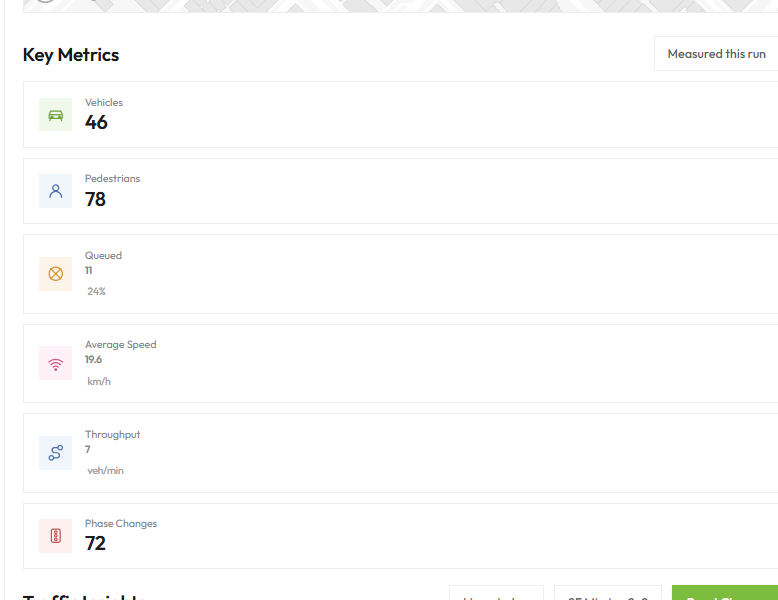
\includegraphics[width=0.98\textwidth,height=0.53\textheight,keepaspectratio]{figures/dashboard-kpis.png}
\caption{Key traffic indicators from the illustrative local SUMO run.}
\label{fig:ui-kpis}
\end{figure}

Figures~\ref{fig:ui-map} and~\ref{fig:ui-kpis} are authentic screenshots captured from
the local frontend during a short demonstration simulation. They illustrate the user
interface only; their transient counters are not included in the 30-episode study or
the aggregate results table.

\begin{figure}[htbp]
\centering
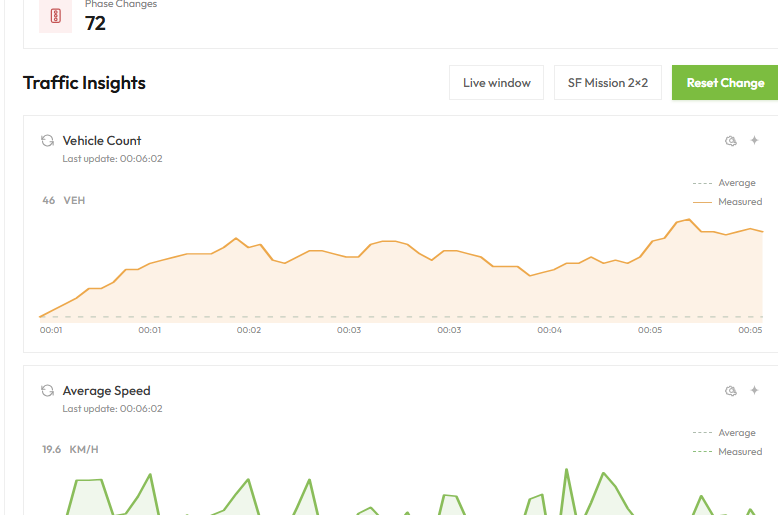
\includegraphics[width=0.98\textwidth,height=0.53\textheight,keepaspectratio]{figures/dashboard-trends.png}
\caption{Live vehicle-count and speed trends in the SUMO dashboard.}
\label{fig:ui-trends}
\end{figure}

\begin{figure}[htbp]
\centering
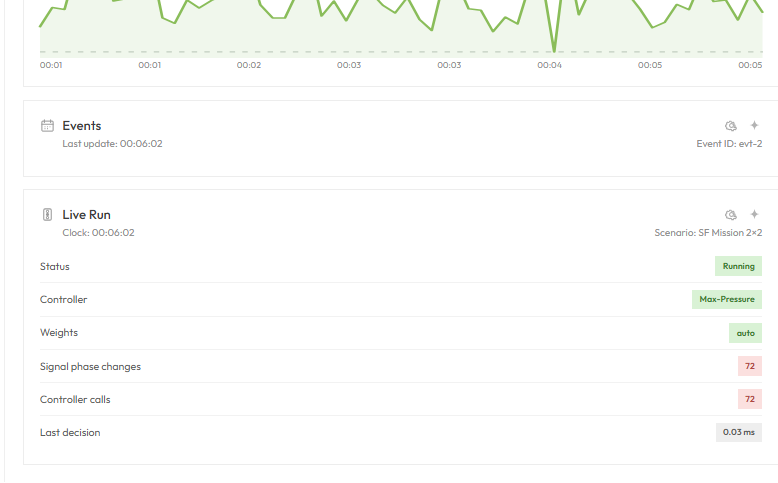
\includegraphics[width=0.98\textwidth,height=0.53\textheight,keepaspectratio]{figures/dashboard-live-run.png}
\caption{Live run details, including the selected controller and signal-phase changes.}
\label{fig:ui-live-status}
\end{figure}

The first four screenshots in this section were captured from the local frontend
during a short demonstration simulation. Their transient counters are not included in
the 30-episode study or the aggregate results table.

\subsection{Project interface and simulation screenshots}
The additional images in the project image collection document complementary parts of
the system. They are included as interface and simulation illustrations, not as
independent measurements. In particular, map tiles, dashboard counters, and event
overlays provide operational context; they do not replace the SUMO episode CSVs used
for the quantitative analysis.

\begin{figure}[htbp]
\centering
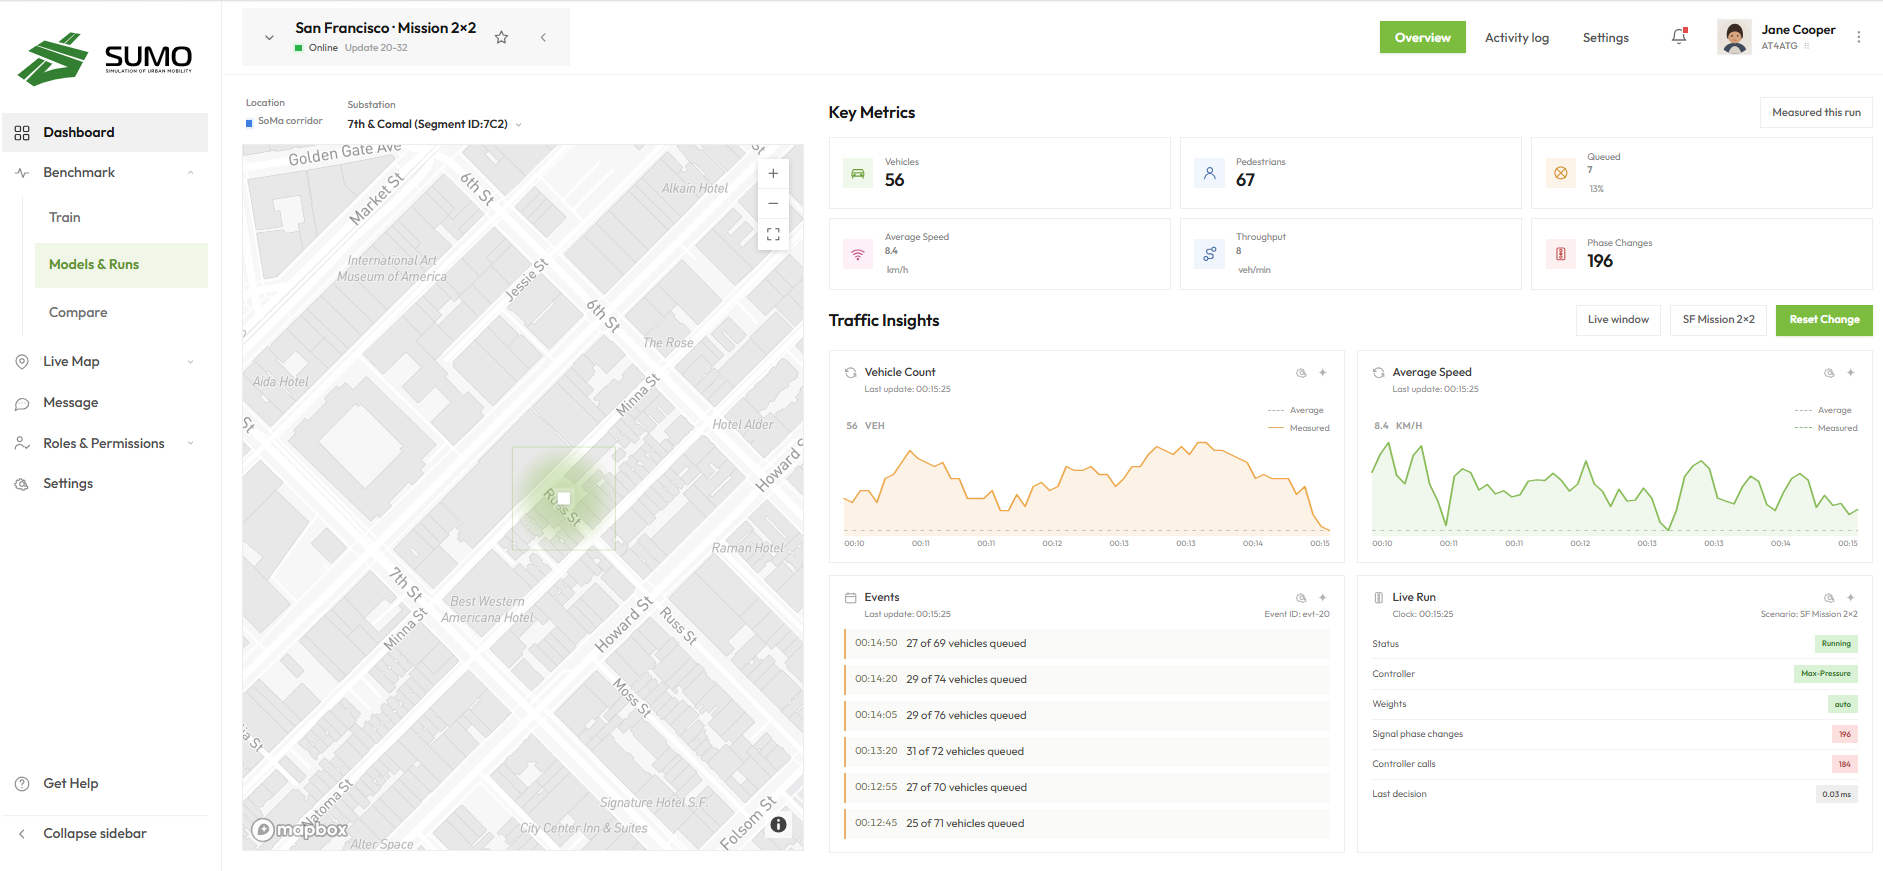
\includegraphics[width=0.98\textwidth,height=0.53\textheight,keepaspectratio]{figures/dashboard.png}
\caption{Project-provided dashboard: map-led overview and traffic status panels.}
\label{fig:provided-dashboard}
\end{figure}

\begin{figure}[htbp]
\centering
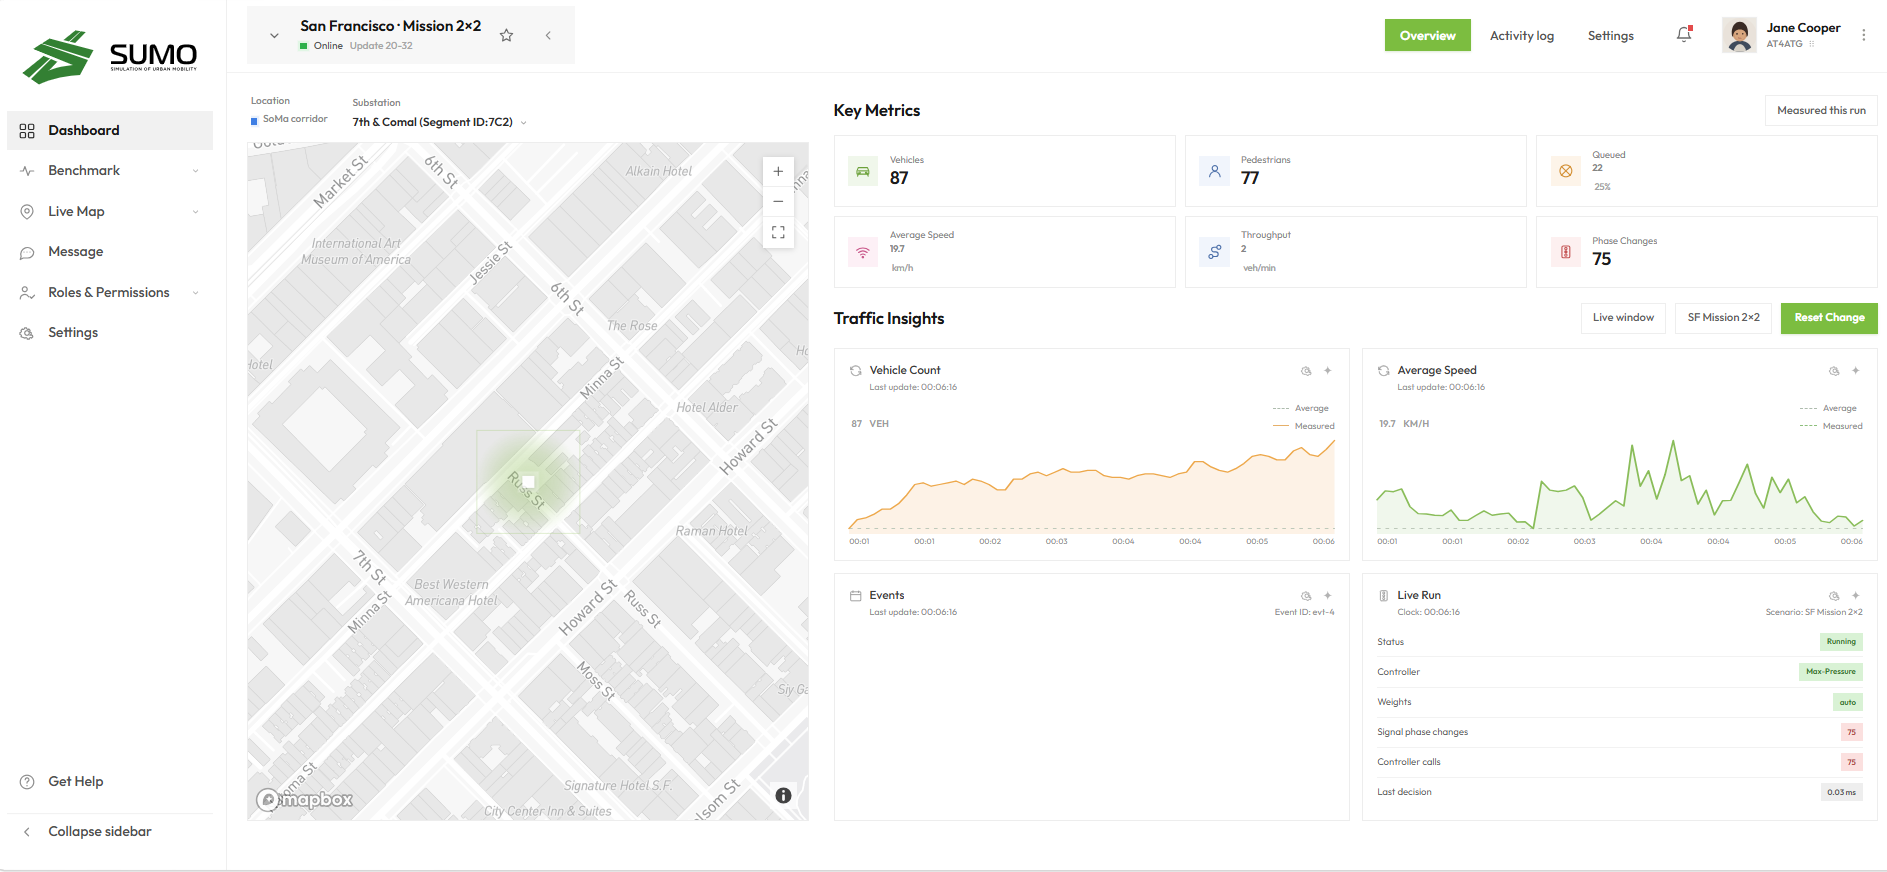
\includegraphics[width=0.98\textwidth,height=0.53\textheight,keepaspectratio]{figures/dashboard2.png}
\caption{Project-provided dashboard: monitoring panels and live control actions.}
\label{fig:provided-dashboard2}
\end{figure}

Figures~\ref{fig:provided-dashboard} and~\ref{fig:provided-dashboard2} show how
simulation status, traffic indicators, and operator controls are brought together.
They help explain the intended user workflow: first inspect the network and current
conditions, then monitor performance and access actions for a running scenario.
Because these supplied screenshots may represent different demo states or interface
iterations, their displayed values should be treated as illustrative UI content.

\begin{figure}[htbp]
\centering
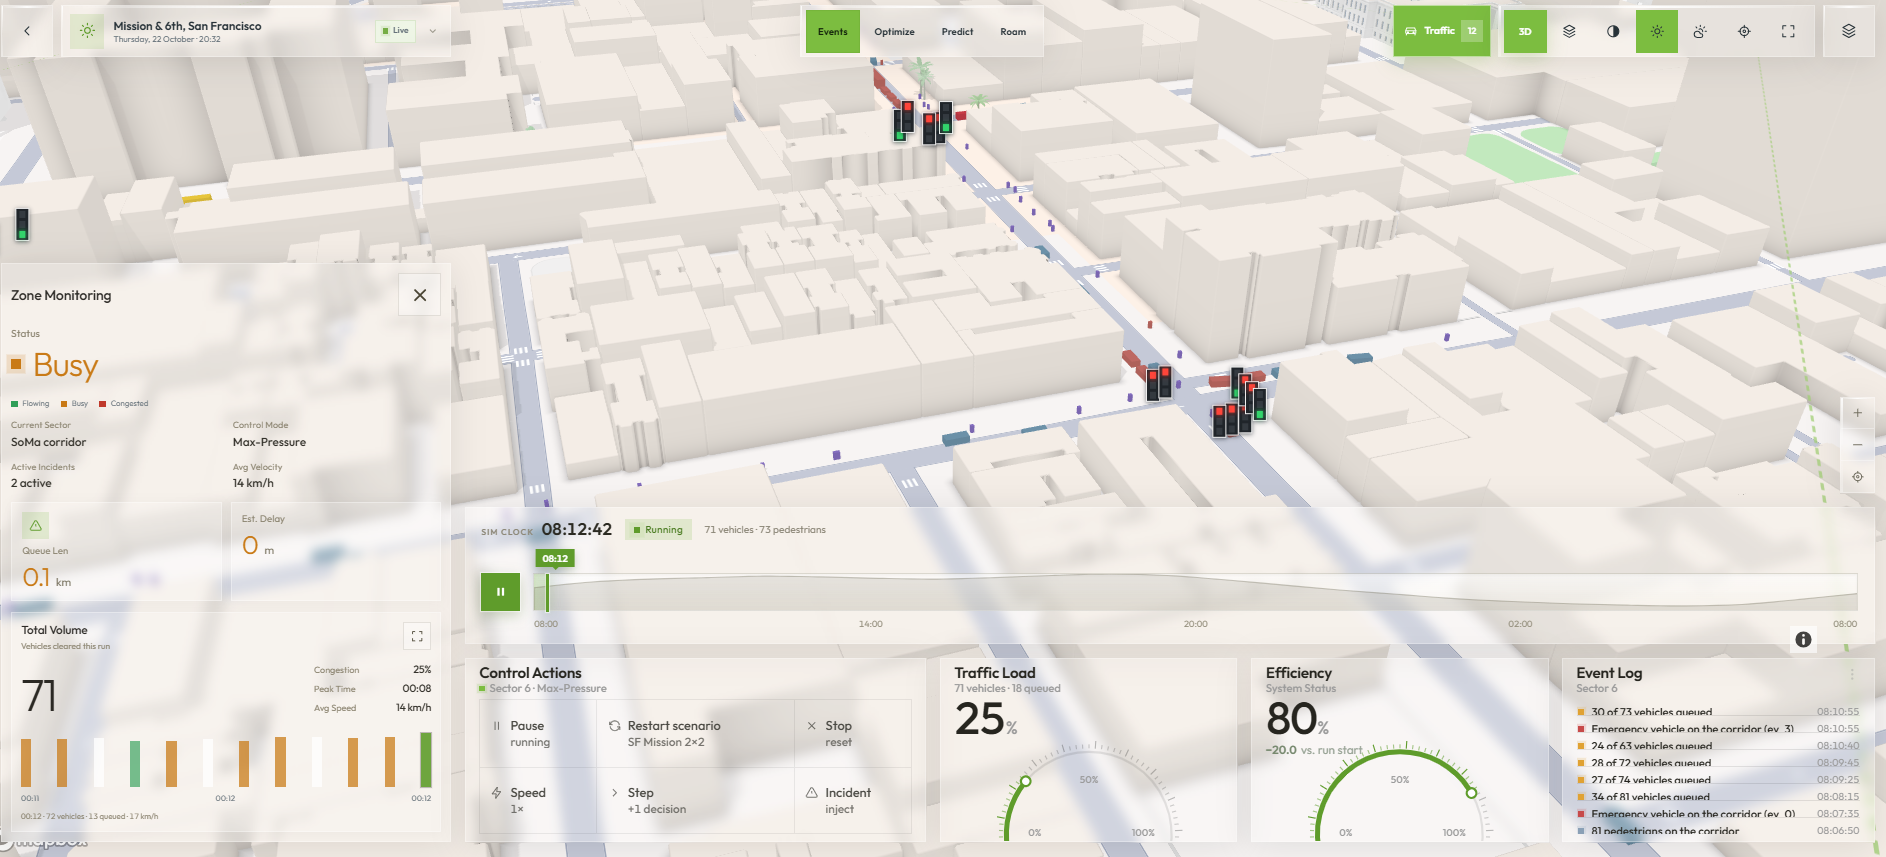
\includegraphics[width=0.98\textwidth,height=0.53\textheight,keepaspectratio]{figures/mapbox.png}
\caption{Mapbox city view with the project traffic-operation overlays.}
\label{fig:mapbox-city}
\end{figure}

\begin{figure}[htbp]
\centering
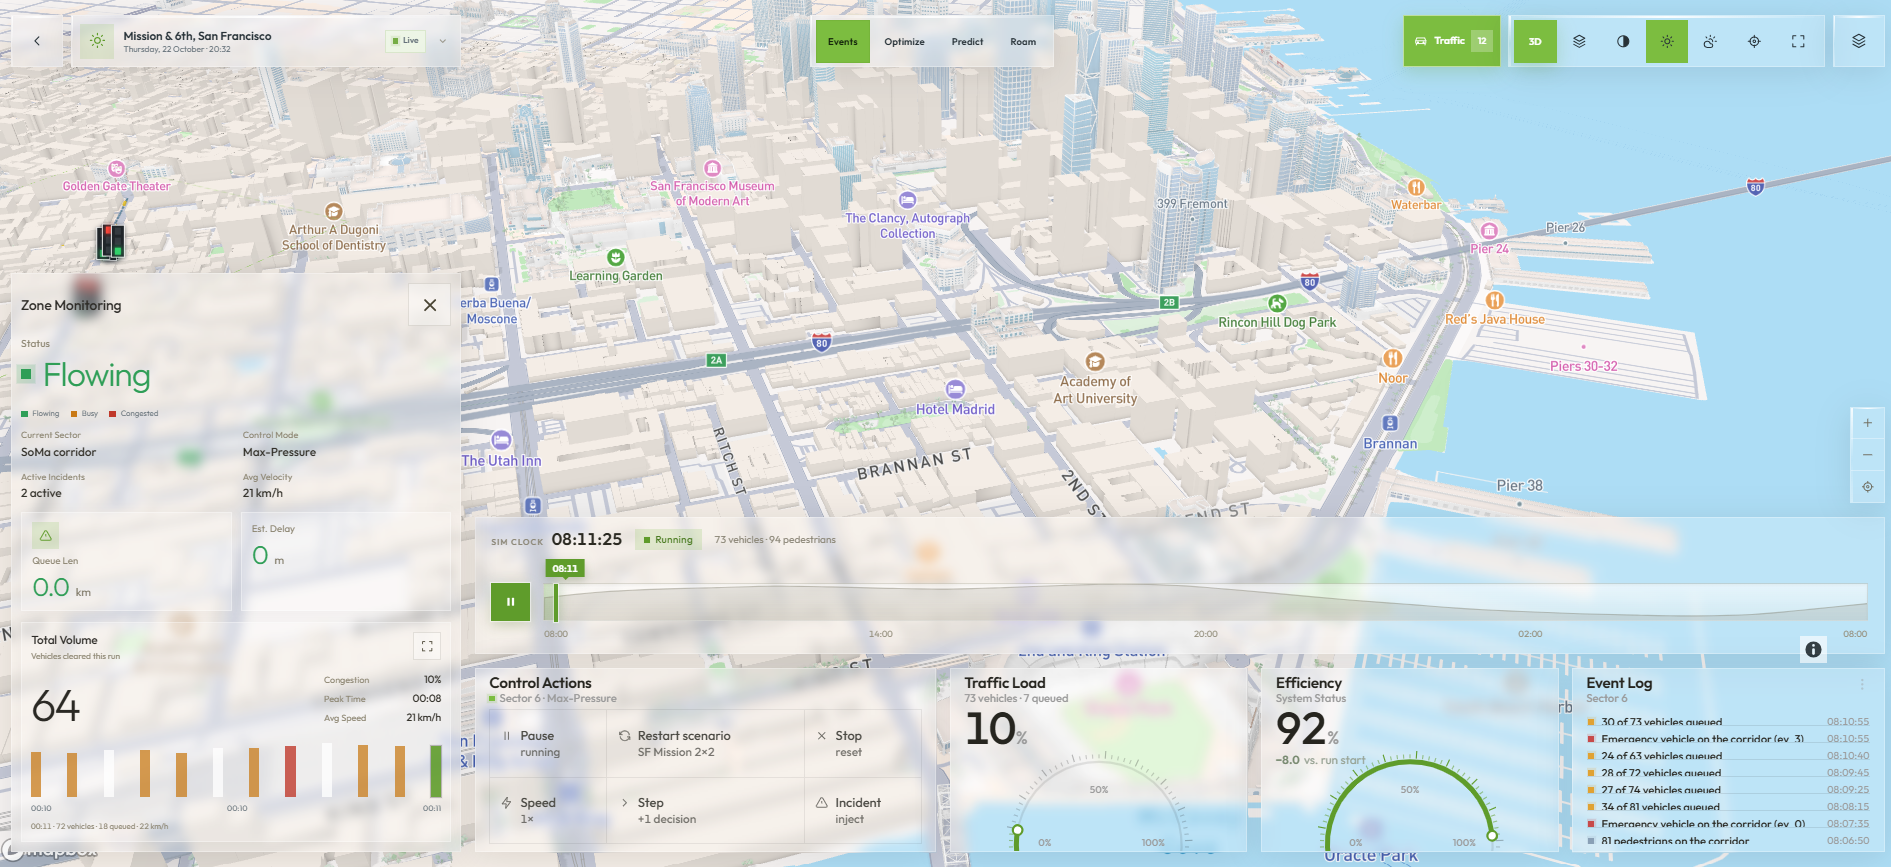
\includegraphics[width=0.98\textwidth,height=0.53\textheight,keepaspectratio]{figures/mapbox2.png}
\caption{Three-dimensional city view with live controls and status panels.}
\label{fig:mapbox-3d}
\end{figure}

The Mapbox views in Figures~\ref{fig:mapbox-city} and~\ref{fig:mapbox-3d} illustrate
two visualisation levels: a broad city context and a closer three-dimensional view
around the monitored corridor. In a deployed workflow, the geographic display can
help an operator locate a corridor or incident, while the simulator remains
responsible for vehicle movement and the study pipeline remains responsible for
quantitative evaluation. A rendered map is not evidence that the underlying
geographic or traffic data are live, calibrated, or externally verified.

\begin{figure}[htbp]
\centering
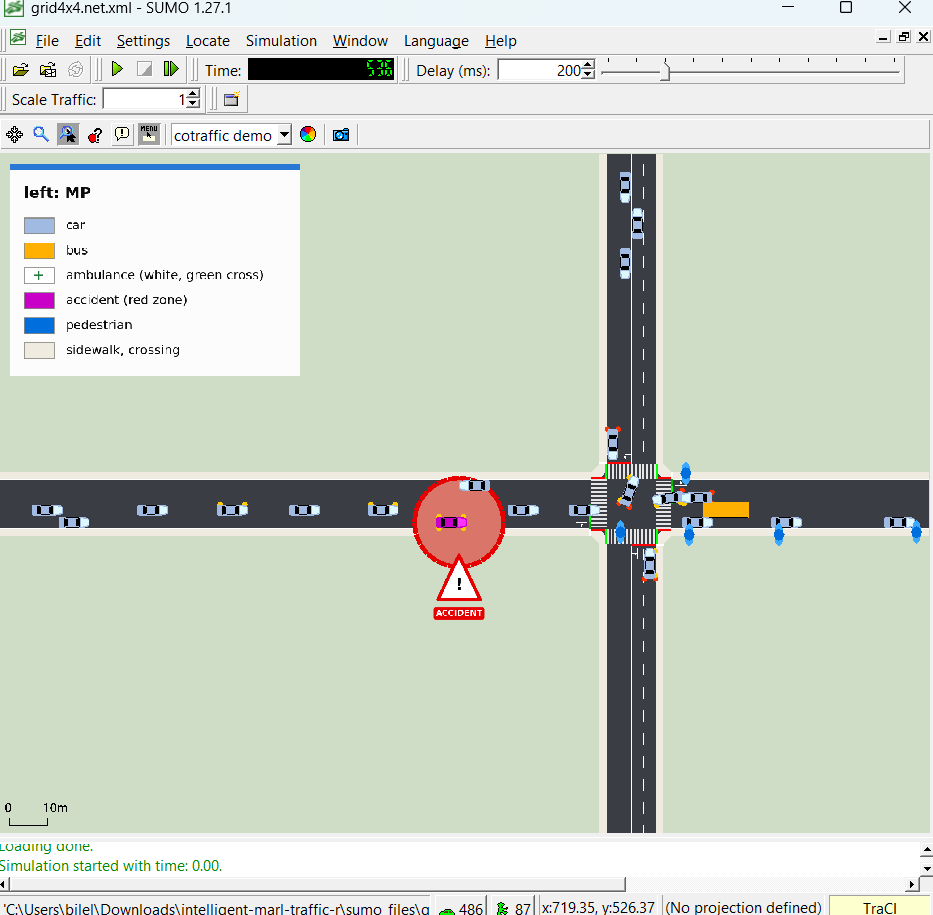
\includegraphics[width=0.98\textwidth,height=0.53\textheight,keepaspectratio]{figures/sumoInterfaceHavingAccident.png}
\caption{SUMO graphical interface displaying an incident-focused simulation view.
This project-provided screenshot illustrates visual monitoring of an incident; it is
not one of the 30 episodes in the baseline comparison.}
\label{fig:sumo-incident}
\end{figure}

Figure~\ref{fig:sumo-incident} complements the web interface with the simulator's own
graphical view. Showing the event in SUMO is useful for qualitative inspection of a
scenario, for example to check that an incident object and nearby road users appear
where expected. Visual inspection is a debugging aid; it cannot establish that the
event schedule, route generation, or controller response is correct without checking
the underlying configuration and run records.

\begin{figure}[htbp]
\centering
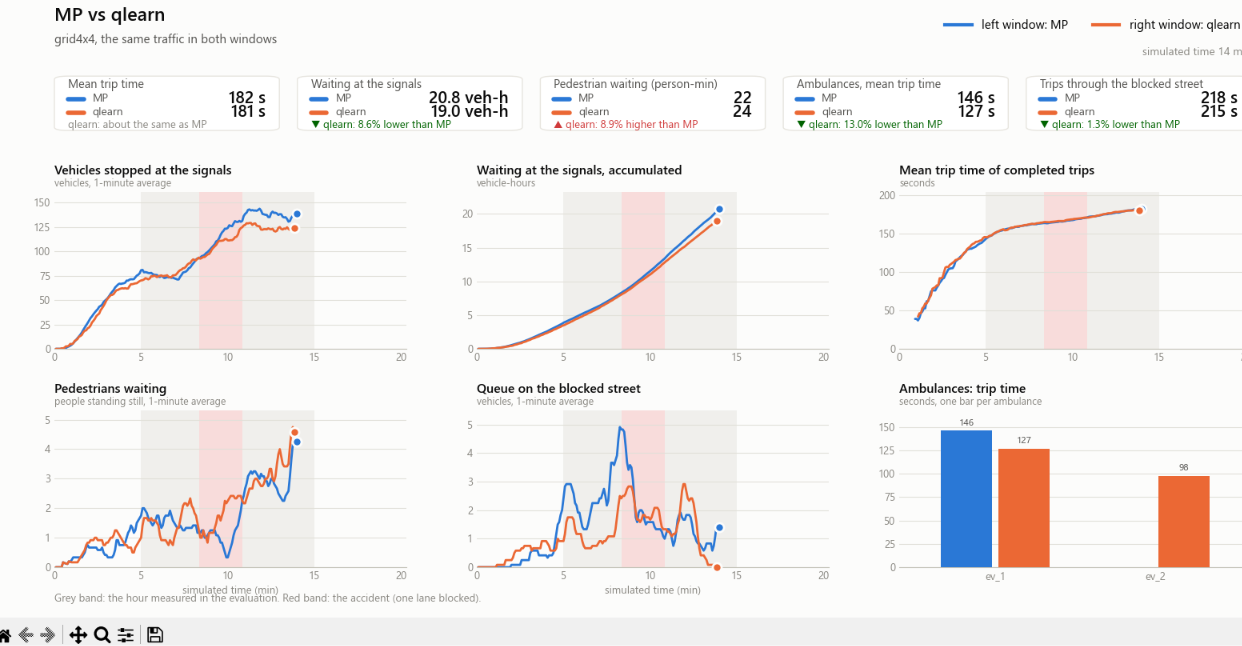
\includegraphics[width=0.98\textwidth,height=0.53\textheight,keepaspectratio]{figures/benchmark.png}
\caption{Supplied benchmark visual labelled ``MP vs qlearn'' on a
\texttt{grid4x4} scenario.}
\label{fig:provided-benchmark}
\end{figure}

\begin{figure}[htbp]
\centering
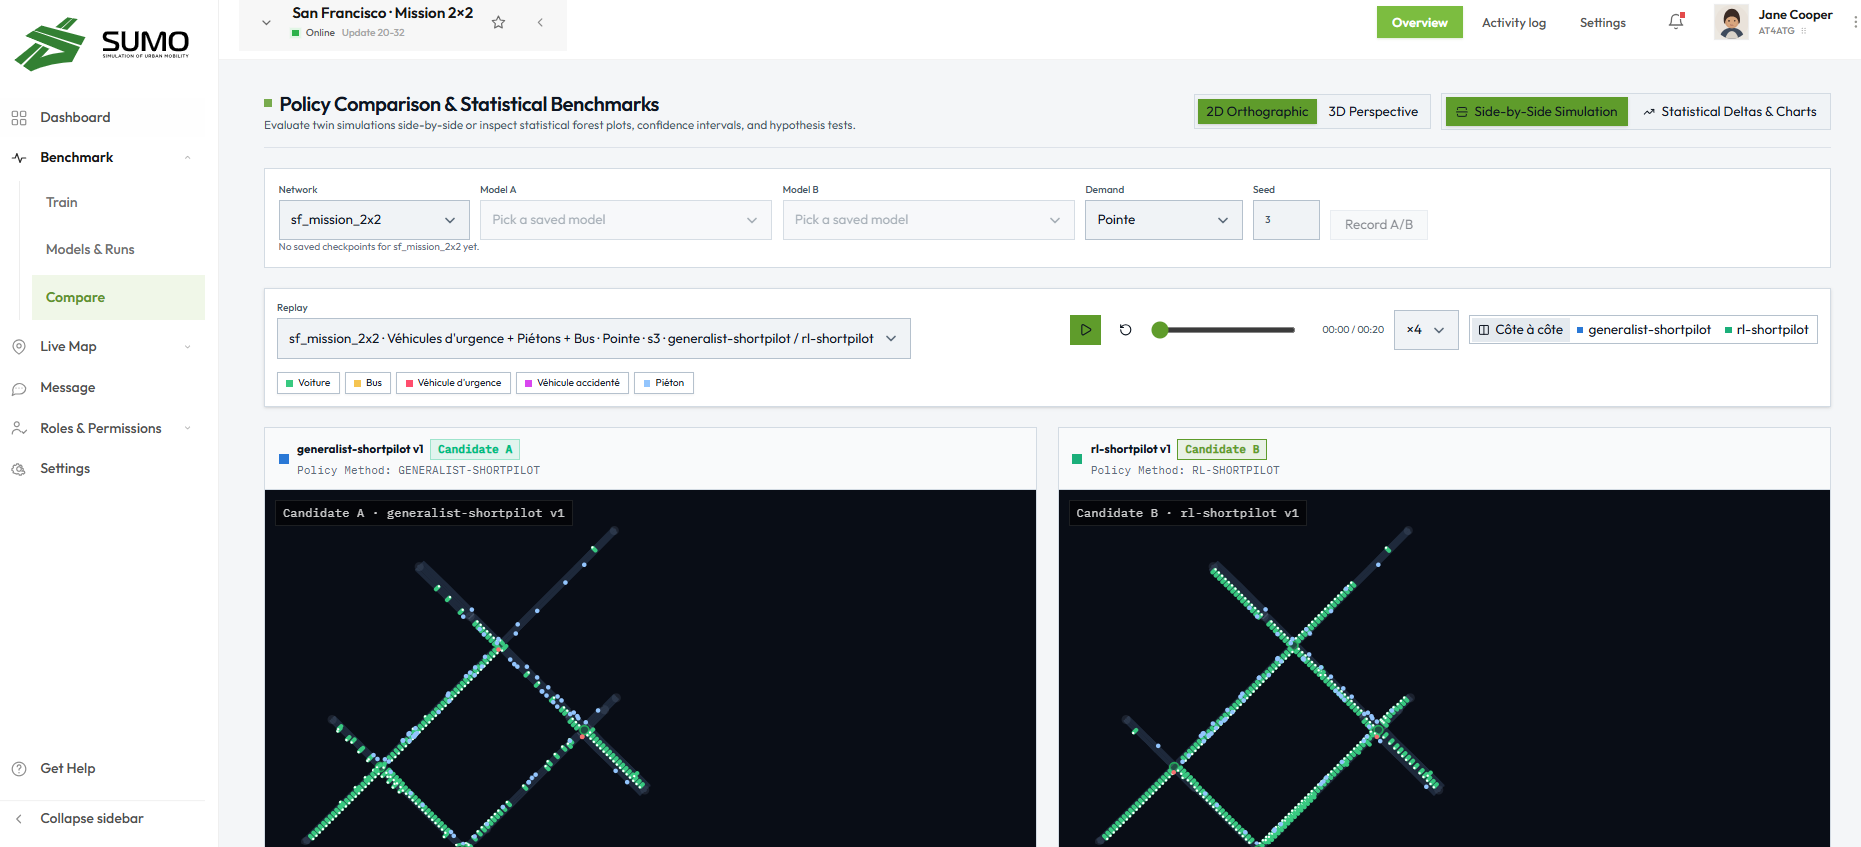
\includegraphics[width=0.98\textwidth,height=0.53\textheight,keepaspectratio]{figures/dashboardcompar.png}
\caption{Dashboard comparison interface for selecting and replaying two
candidate policies.}
\label{fig:provided-compare}
\end{figure}

Figures~\ref{fig:provided-benchmark} and~\ref{fig:provided-compare} show the project's
benchmarking concept: compare candidate policies on the same simulated demand and
inspect a collection of service metrics, rather than relying on a single headline
score. The supplied \texttt{benchmark.png} depicts a separate grid4x4 MP--qlearn
visualisation, while the numerical pilot in this report is a three-controller
comparison on \texttt{grid2x2}. The raw run-level records for the screenshot's
MP--qlearn values are not part of the pilot CSV set documented here. Consequently,
those image values are not quoted, recomputed, or combined with the results in
Section~\ref{sec:results}. Similarly, the comparison-page screenshot documents the
frontend workflow; it should not be read as proof that the displayed candidate
checkpoints were available or that an A/B run completed successfully.

\subsection{Reproducibility artifacts}
The following project files preserve the reported pilot:
\begin{itemize}
  \item \texttt{configs/experiments/technical\_report\_quick.yaml} - matrix definition.
  \item \texttt{docs/technical\_report\_metrics.csv} - one row per completed episode.
  \item \texttt{docs/technical\_report\_results\_summary.csv} - across-seed means,
  standard deviations, and paired deltas.
  \item \texttt{docs/technical\_report\_experiment\_manifest.json} - commit, software
  versions, protocol, seeds, run count, and caveats.
\end{itemize}

\section{Results}
\label{sec:results}
\subsection{Primary outcome: mean waiting time}
The actuated controller had the lowest mean waiting time in both event settings.
Against Max-Pressure, its seed-paired mean difference was
$-2.08 \pm 0.70$ seconds in the normal scenario and
$-2.13 \pm 0.63$ seconds in the emergency scenario (mean $\pm$ sample SD of paired
differences). These correspond to approximately 24\% lower mean waiting than
Max-Pressure in this particular pilot. Fixed-time produced the highest mean waiting
time, at about 13.0 seconds in both scenarios.

\begin{table}[htbp]
\centering\small
\caption{Mean waiting time by controller and scenario (seconds; across-seed mean
$\pm$ sample standard deviation, $n=5$).}
\begin{tabular}{lcc}
\toprule
\textbf{Controller} & \textbf{Normal} & \textbf{Emergency} \\
\midrule
Fixed-time (\texttt{ft}) & $13.02 \pm 0.98$ & $13.01 \pm 1.17$ \\
Actuated (\texttt{act}) & $\mathbf{6.69 \pm 0.62}$ & $\mathbf{6.72 \pm 0.50}$ \\
Max-Pressure (\texttt{mp}) & $8.77 \pm 1.04$ & $8.85 \pm 0.63$ \\
\bottomrule
\end{tabular}
\end{table}

\subsection{Trade-offs across metrics}
Max-Pressure had the lowest mean CO$_2$ intensity, while actuated control achieved the
lowest delay and 95th-percentile waiting time. Max-Pressure's throughput advantage
over actuated control was small: 8.4 vehicles per hour in normal demand and 2.4
vehicles per hour in the emergency condition. These differences are descriptive;
they should not be interpreted as statistically reliable. The results suggest that a
controller choice depends on the objective weights and operating priorities, rather
than one metric alone.

\begin{figure}[htbp]
\centering
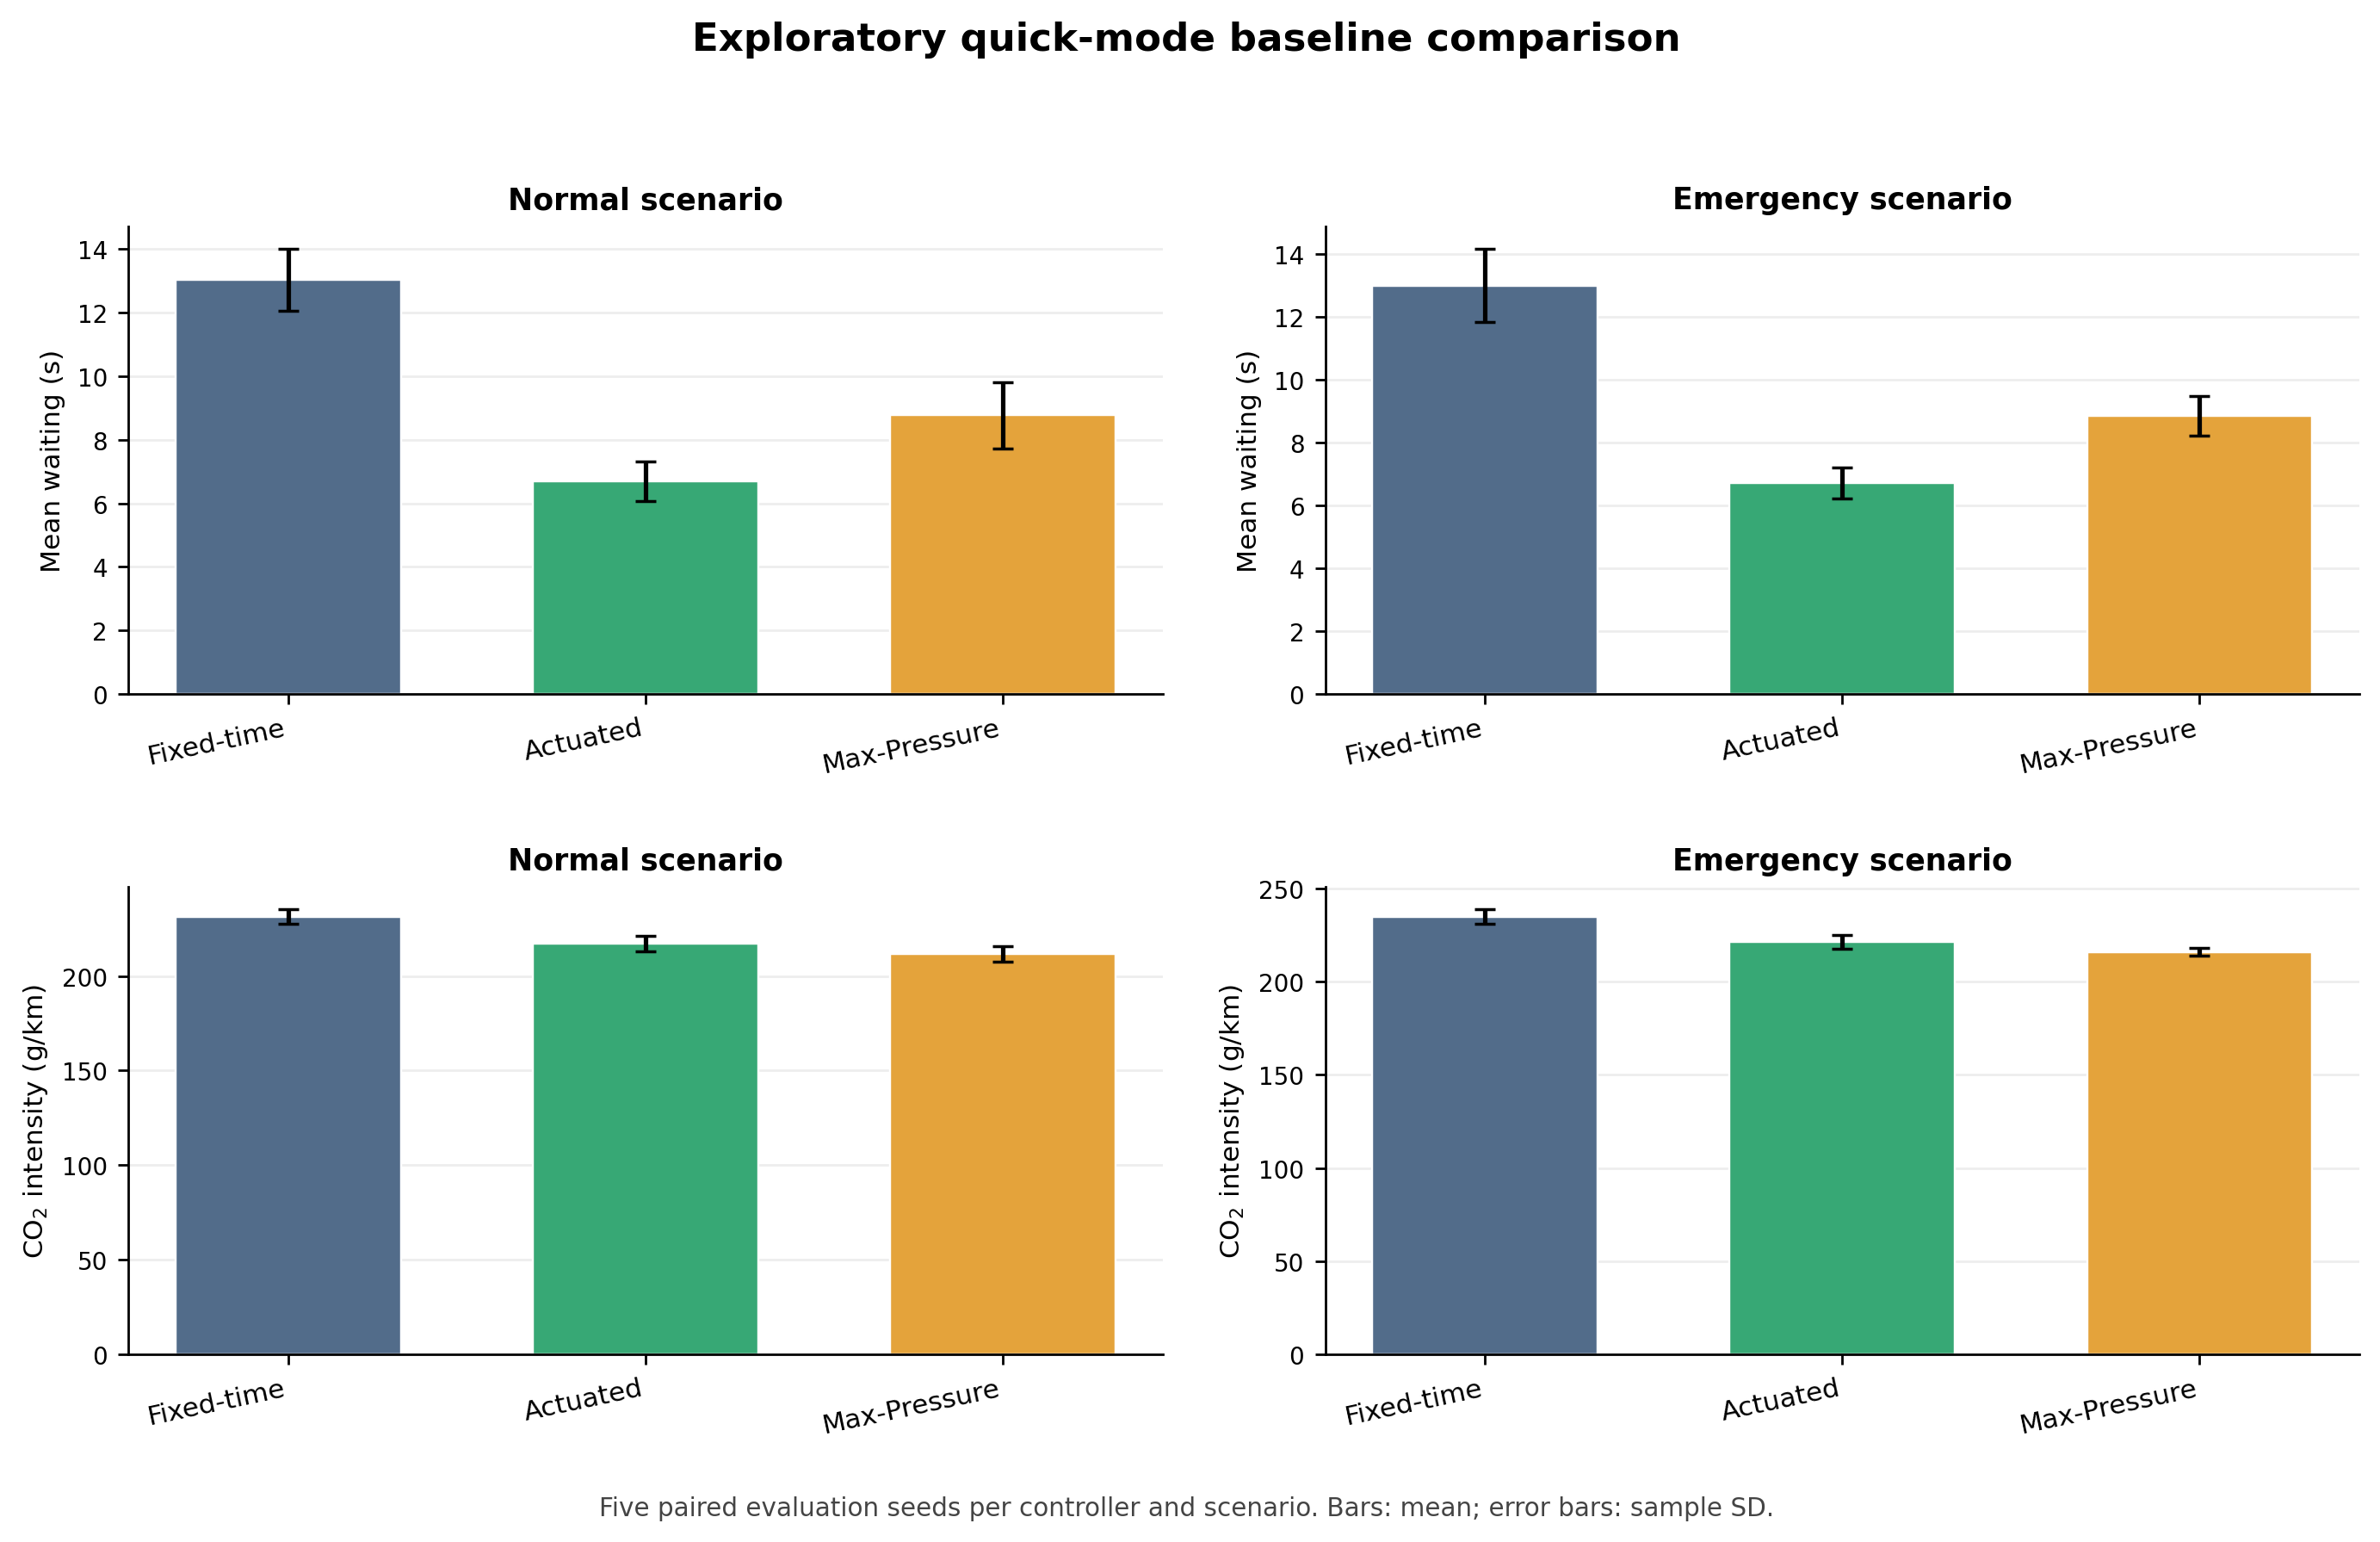
\includegraphics[width=0.94\textwidth]{figures/baseline-comparison.png}
\caption{Pilot comparison for mean waiting time and CO$_2$ intensity. Bars show
across-seed means; error bars show sample standard deviation across five seeds. The
error bars describe variability and are not confidence intervals.}
\label{fig:baseline-results}
\end{figure}

\begin{table}[htbp]
\centering\small
\caption{Additional service and emissions outcomes (mean $\pm$ sample SD).}
\begin{tabular}{llccc}
\toprule
\textbf{Scenario} & \textbf{Metric} & \textbf{Fixed-time} & \textbf{Actuated} & \textbf{Max-Pressure} \\
\midrule
Normal & Travel time (s) & $85.47\pm1.49$ & $78.39\pm2.10$ & $78.63\pm1.94$ \\
Normal & 95th-percentile wait (s) & $31.47\pm1.60$ & $18.45\pm1.30$ & $31.19\pm3.58$ \\
Normal & Throughput (veh/h) & $956.4\pm50.8$ & $966.0\pm41.1$ & $974.4\pm48.3$ \\
Normal & Mean queue (veh) & $3.37\pm0.35$ & $1.70\pm0.17$ & $2.28\pm0.35$ \\
Normal & CO$_2$ (g/km) & $231.37\pm3.78$ & $217.22\pm4.11$ & $\mathbf{211.73\pm4.11}$ \\
\midrule
Emergency & Travel time (s) & $85.18\pm1.66$ & $78.16\pm1.98$ & $78.56\pm1.38$ \\
Emergency & 95th-percentile wait (s) & $31.99\pm2.08$ & $18.08\pm2.26$ & $30.72\pm2.57$ \\
Emergency & Throughput (veh/h) & $980.4\pm49.8$ & $994.8\pm49.9$ & $997.2\pm51.2$ \\
Emergency & Mean queue (veh) & $3.45\pm0.40$ & $1.76\pm0.13$ & $2.35\pm0.21$ \\
Emergency & CO$_2$ (g/km) & $234.86\pm3.83$ & $221.29\pm3.90$ & $\mathbf{215.82\pm2.11}$ \\
\bottomrule
\end{tabular}
\end{table}

\subsection{Operational checks}
Across the 30 pilot episodes, the run-level CSV records zero collisions, zero
teleported vehicles, zero unfinished trips, and zero vehicles that were never inserted.
These are simulator outcome checks for this short experiment, not a safety guarantee.
Mean vehicles represented were 161.8 per episode in the normal scenario and 166.6 in
the emergency scenario; the same seed set produced the same total vehicle counts
across the compared controllers in each scenario.

\subsection{Interpretation}
Within the study boundary, actuated control provides a useful delay-oriented
reference: it improved mean and tail waiting relative to both other controllers, but
its emissions intensity was about 2.5--2.6\% higher than Max-Pressure. The fixed-time
plan was competitive only on simplicity; it produced substantially higher delay and
queueing in this short run. Because the network is small, the demand is simulated, and
the sample is limited, these observations are a basis for a larger experiment, not a
conclusion about city-wide controller performance.

\section{Software Validation and Reproducibility}
\subsection{Validation performed}
The associated experiment manifest records the following checks on the project
environment:
\begin{itemize}
  \item Python test suite: \textbf{208 passed}; one Starlette/httpx deprecation warning.
  \item Frontend unit tests: \textbf{5 passed} with Vitest.
  \item Frontend production build: \textbf{passed}; existing dependency-annotation and
  large-bundle warnings were reported.
  \item Pilot experiment: \textbf{30 of 30 episodes completed}.
\end{itemize}

The recorded environment is Python 3.11.9 and Eclipse SUMO 1.27.1. Test collection on
Python 3.10.11 was not successful because \texttt{api/jobs.py} imports
\texttt{datetime.UTC}, which is unavailable in Python 3.10. This compatibility gap is
reported rather than silently treating that interpreter as validated.

\subsection{Reproduction}
From the repository root, with SUMO installed and the Python dependencies available,
the pilot matrix can be rerun with:
\begin{quote}\small\ttfamily
.venv\textbackslash Scripts\textbackslash python.exe -m cotraffic evaluate
--experiment technical\_report\_quick --methods baselines --jobs 1
\end{quote}
The command resolves the configuration in \texttt{configs/experiments/}; use the
project's normal network-generation step first if the generated network assets are
missing. After evaluation, use the project's aggregate command to refresh summary
tables. The checked-in report CSV and manifest preserve the exact run evidence used
here.

\section{Limitations, Ethics, and Deployment Considerations}
\subsection{Evidence limitations}
\begin{itemize}
  \item \textbf{Short horizon:} quick mode measures 600 seconds after a 300-second
  warm-up, rather than the full one-hour measured protocol.
  \item \textbf{Small sample:} five seeds per scenario are insufficient for strong
  statistical claims; no inferential tests or confidence intervals were run.
  \item \textbf{Limited environment:} one generated 2-by-2 network and one medium
  demand level do not represent network diversity or peak conditions.
  \item \textbf{Controller scope:} the reported comparison excludes PPO, DQN, LLM, and
  specialised emergency/pedestrian policies.
  \item \textbf{Simulation validity:} vehicle demand, routes, driver behaviour, and
  emissions depend on SUMO configuration; they are not calibrated field measurements.
  \item \textbf{Interface boundary:} the captured live demonstration is a separate
  session and must not be substituted for the saved paired experiment.
\end{itemize}

\subsection{Ethics and responsible use}
The pilot contains synthetic traffic only and does not process personal data. Before
any real deployment, the team would need to validate the network and demand against
authorised local data, document privacy and retention controls, assess pedestrian and
emergency-service impacts, and obtain review by relevant transportation authorities.
Controller decisions should remain auditable and subject to human operational
oversight. A simulation-only zero-collision result is not evidence that a system is
safe for public roads.

\subsection{Operational security}
Provider credentials and Mapbox tokens are configured locally and are not embedded
in this report. A deployment review should additionally assess authentication,
authorisation, secret management, CORS policy, service exposure, logging, and
provider data handling. The current dashboard is a research/demo interface and is
not asserted to meet production security or reliability requirements.

\subsection{Generative AI disclosure}
Generative AI assistance was used to help organise and edit this technical report.
Project-specific statements and numerical values were checked against the repository,
experiment configuration, stored CSV outputs, manifest, and executed validation
results. The project authors remain responsible for reviewing, correcting, and
approving the final submission. This statement should be adjusted by the team if it
does not accurately describe all tools used during project work..

\section{Conclusion and Future Work}
This project provides an end-to-end traffic-control research scaffold: SUMO-based
simulation, multi-agent control interfaces, a safety shield, classical baselines, a
parameter-shared PPO training path, a FastAPI integration layer, and a live dashboard.
The measured pilot establishes a small, reproducible comparison rather than an
unsupported learned-policy success claim. In this sample, actuated control led on
waiting time and queueing, while Max-Pressure achieved the lowest CO$_2$ intensity and
slightly higher throughput.

The next experiment should use the full evaluation horizon, a substantially larger
paired seed set, and multiple networks and demand levels. It should include the
trained generalist PPO checkpoint, confirm that checkpoint selection is separated
from evaluation seeds, and report paired uncertainty intervals and appropriate
statistical tests. Emergency, pedestrian, and emissions outcomes should be examined
explicitly, with ablations to identify which observation and reward components drive
any differences. Only after simulator calibration and independent validation should
the team consider a field-oriented pilot.

\section*{References}
\addcontentsline{toc}{section}{References}
\begin{enumerate}[label={[\arabic*]},leftmargin=2.1em]
  \item M. Behrisch, L. Bieker, J. Erdmann, and D. Krajzewicz,
  ``SUMO - Simulation of Urban MObility: An Overview,'' in
  \emph{Proceedings of the SIMUL 2011}, 2011.
  \item F. V. Webster, \emph{Traffic Signal Settings}, Road Research Technical Paper
  No. 39, Road Research Laboratory, London, 1958.
  \item P. Varaiya, ``The Max-Pressure Controller for Arbitrary Networks of Signalized
  Intersections,'' \emph{Transportation Research Part C: Emerging Technologies},
  vol. 36, pp. 177--195, 2013.
  \item J. Schulman, F. Wolski, P. Dhariwal, A. Radford, and O. Klimov,
  ``Proximal Policy Optimization Algorithms,'' arXiv:1707.06347, 2017.
  \item J. Terry et al., ``PettingZoo: Gym for Multi-Agent Reinforcement Learning,''
  in \emph{Advances in Neural Information Processing Systems, Datasets and
  Benchmarks Track}, 2021.
  \item Esprit School of Engineering 5DS8 Project Team,
  \emph{Intelligent Multi-Agent Urban Traffic Management: Source Code and
  Experiment Artifacts}, repository documentation and configuration files.
\end{enumerate}

\appendix
\section{Pilot Evidence Files}
The following artifacts should be submitted or kept alongside the report so that
reviewers can inspect the basis of the reported values:
\begin{itemize}
  \item \texttt{docs/technical\_report\_metrics.csv} - 30 episode-level records.
  \item \texttt{docs/technical\_report\_results\_summary.csv} - six controller/scenario
  aggregates and paired differences.
  \item \texttt{docs/technical\_report\_experiment\_manifest.json} - experiment
  provenance and validation notes.
  \item \texttt{configs/experiments/technical\_report\_quick.yaml} - rerun matrix.
  \item \texttt{docs/latex\_report/figures/} - frontend captures, the supplied SUMO
  incident and benchmark images, and the plotted experiment summary used in this
  document.
\end{itemize}

\section{Metric Reading Guide}
\begin{description}[leftmargin=4.2cm,style=nextline]
  \item[Mean waiting time] Episode-level mean vehicle waiting time, in seconds; lower
  is better for delay.
  \item[95th-percentile waiting] Upper-tail waiting measure; it describes the 95th
  percentile of vehicle waiting in the episode and is not a confidence bound.
  \item[Mean queue] Episode-level average queue measure in vehicles.
  \item[Throughput] Completed vehicles scaled to vehicles per hour for the measured
  interval; it is not a count of all scheduled trips.
  \item[CO$_2$ intensity] Emission output normalised by distance travelled, in grams
  per kilometre, from the configured SUMO emissions model.
  \item[Mean $\pm$ SD] Across-seed sample mean and sample standard deviation. For
  paired differences, the SD is computed over the five seed-wise differences.
\end{description}

\section{Study-to-Claim Boundary}
\begin{center}
\begin{tabularx}{0.96\textwidth}{>{\bfseries}p{4.0cm}X}
\toprule
Supported by this report & Not supported by this report \\
\midrule
The three classical controllers produced the reported descriptive outcomes on
\texttt{grid2x2}, medium demand, and five seeds per scenario. &
That actuated control is universally best, or that any difference is statistically
significant. \\
The specified local simulation recorded no collisions, teleports, unfinished trips,
or never-inserted vehicles in these episodes. &
That a deployed traffic system is safe, fair, robust, or improves real-world traffic. \\
The repository provides a PPO training and inference path and a configured generalist
recipe. &
That PPO outperforms the classical baselines in this pilot; it was not compared here. \\
\bottomrule
\end{tabularx}
\end{center}

\end{document}
